\newpage

\section{Problem 6 (8 pts)}
\subsection{Answer}

Consider the relation \textit{``is a subtype of''} as $R$ over the set $A = \{ rectangle, quadrilateral, square, \\parallelogram,rhombus\}$.
\\

$
R = \{(rectangle, quadrilateral), (rectangle, parallelogram), (square, rectangle),
\\(square, quadrilateral), (parallelogram, quadrilateral), (rhombus, quadrilateral),
\\(rhombus, parallelogram), (rectangle, rectangle), (quadrilateral, quadrilateral),
\\(square, square), (parallelogram, parallelogram), (rhombus, rhombus)\}
$
\\ \begin{enumerate}
    \item In order for a relation to be an equivalence relation, it must be reflexive, symmetric and transitive.
    \begin{itemize}
        \item $R$ is reflexive since every element in $A$ is related to itself. That is, $\forall a \in A: aRa$. 
        \item $R$ is not symmetric since $(rectangle, quadrilateral) \in R, but (quadrilateral, rectangle) \notin R.$
        \item $R$ is transitive since for elements $a, b, c$ in the set $A$, if $a$ and $b$ are related by $R$, and $b$ and $c$ are related by $R$, then $a$ and $c$ are also related by $R$. That is, $\forall a,b,c \in A: (aRb \wedge bRc) \rightarrow aRc$.
    \end{itemize}
    Since the relation is reflexive, transitive, but not symmetric, it is not an equivalence relation.
    
    \item In order for a relation to be a partial order relation, it must be reflexive, antisymmetric and transitive.
    \begin{itemize}
        \item R is antisymmetric since for elements $a, b$ in the set $A$, if $aRb$ and $bRa$, then $a=b$. In other words, there is no pair in R such that the reverse of this pair exists, unless the pair contains identical elements.
    \end{itemize}
    From the previous point, it has been concluded that $R$ is reflexive and transitive. Since $R$ is also antisymmetric, it is a partial order.
    \\
    \\
    The Hasse diagram of $R$ is shown in the following figure:
    \newpage
    \begin{figure}[h]
        \centering
        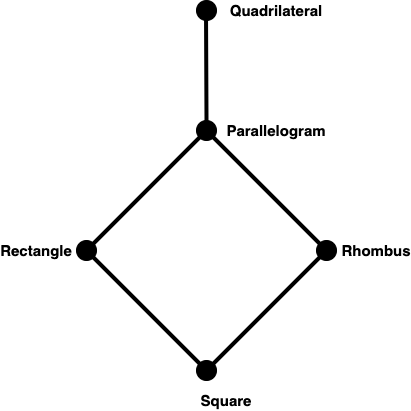
\includegraphics[scale=0.5]{Hasse}
        \caption{Hasse Diagram for Problem 6}
        \label{fig:Hasse}
    \end{figure}
    From figure \ref{fig:Hasse}, it can be concluded that the maximal element is $Quadrilateral$, since it does not have any successors, and the minimal element is $Square$, since it does not have any predecessors.
    
\end{enumerate}